

\section{Background}

\subsection{Large Language Models (LLM)}

The are three different architectures for Large Language Models, encoder-only, decoder-only, and encoder-decoder. Each one has advantages on specific tasks. In Figure \ref{architecture}

\subsubsection{Encoder-only models}
These models are like BERT.
This type of model predict by masking specific words in a sentence.
They are better for classification and sentiment analysis.

\subsubsection{Decoder-only models}
For these model we have the well known GPT-3.
They receive one input and try to predict the entire text.
They are good for summarizing and text-generation.

\subsubsection{Encoder-Decoder models}
T5 is an encoder-decoder models.
They mask entire sequences of text.
Good for translation and question and answering.

\begin{figure}[!ht]
    \centering
        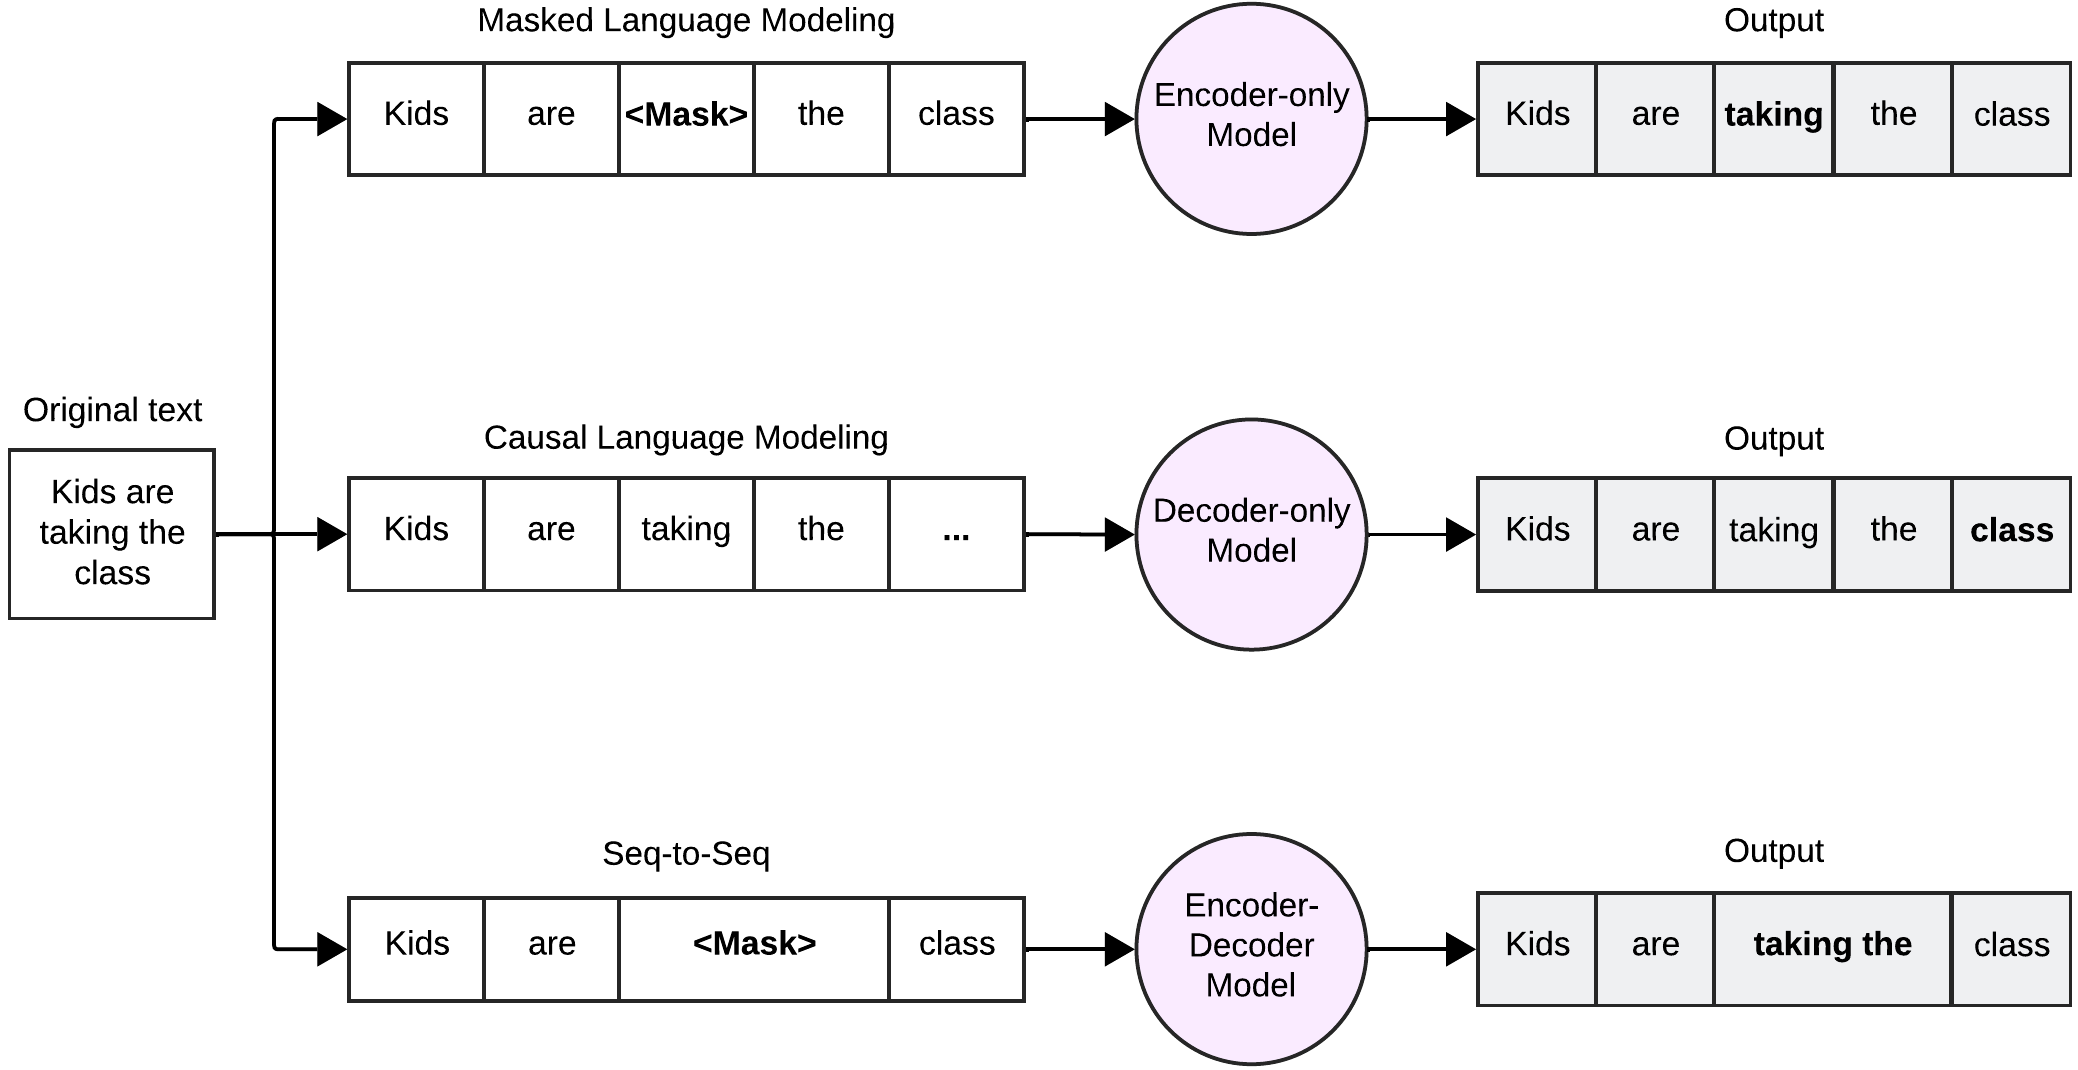
\includegraphics[width=0.5\textwidth]{figures/LLM_Arch_text_generation.png}
        \caption{The transformer architecture}
        \label{architecture}
\end{figure}

